\section{Eliminazione delle generalizzazioni}\label{sec:generalizations}
Di seguito viene mostrato come le generalizzazioni sono state eliminate per produrre
il {\it diagramma E-R ristrutturato}.

Nella totalità dei casi le generalizzazioni sono state eliminate {\bf accorpando
le entità figlie sull'entità padre}.

\vspace{15pt}

Nel caso della generalizzazione che coinvolge le entità {\tt Strumento}, {\tt Macchinario}
e {\tt Attrezzatura}, risulta comodo l'accorpamento sul padre in quanto le entità figlie
non hanno attributi che il padre non possiede e non hanno associazioni con altre entità.

\vspace{5pt}\centerline{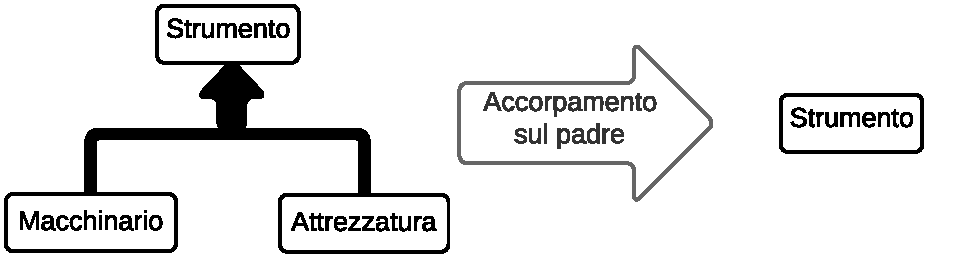
\includegraphics[width=\textwidth]{gen-strumento}}

\vspace{15pt}

Nel caso della generalizzazione che coinvolge le entità {\tt Menu} e  {\tt MenuPassato},
l'accorpamento sul padre non porta all'aggiunta di alcun attributo opzionale (l'attributo
{\tt DataFine} è specificato al momento dell'inserimento del menu nel database, per la business
rule \ref{br.menuenddate} - grazie a questa business rule si evita l'aggiunta di un attributo {\it nullable}).

\vspace{5pt}\centerline{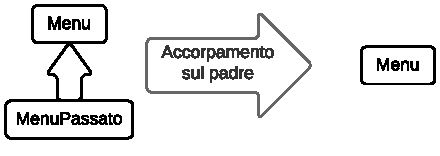
\includegraphics[width=0.8\textwidth]{gen-menu}}

\vspace{15pt}

Nel caso della generalizzazione che coinvolge le entità {\tt Fase}, {\tt FaseIngrediente}
e {\tt FaseManovra}, l'accorpamento sul padre porta all'introduzione di diversi attributi
opzionali: {\tt Durata}, {\tt Testo} ma anche {\tt Dose} e {\tt Primario} in quanto l'associazione
{\tt Aggiunta} diventa opzionale. Non è necessario inserire qui un attributo {\tt Tipo} per
riconoscere il tipo di fase in quanto può essere facilmente dedotto dalla presenza o meno
dell'associazione {\tt Aggiunta}.

\vspace{5pt}\centerline{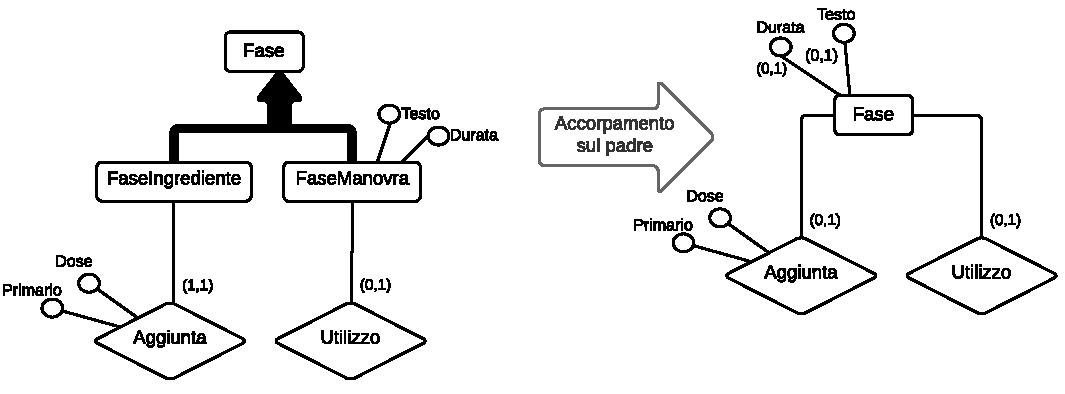
\includegraphics[width=\textwidth]{gen-fase}}

\vspace{15pt}

Nel caso della generalizzazione che coinvolge le entità {\tt Variazione}, {\tt VariazionePiatto}
e {\tt Suggerimento}, l'accorpamento sul padre porta all'aggiunta dell'attributo opzionale
{\tt Nome}. L'associazione {\tt InvioSug} diventa opzionale (e la rinominiamo in {\tt Suggerimento}).
Non è necessario inserire qui un attributo {\tt Tipo} per riconoscere il tipo di variazione
in quanto può essere facilmente dedotto dalla presenza o meno dell'associazione {\tt Suggerimento} (\hbox{ex-\texttt{InvioSug}}).

\vspace{5pt}\centerline{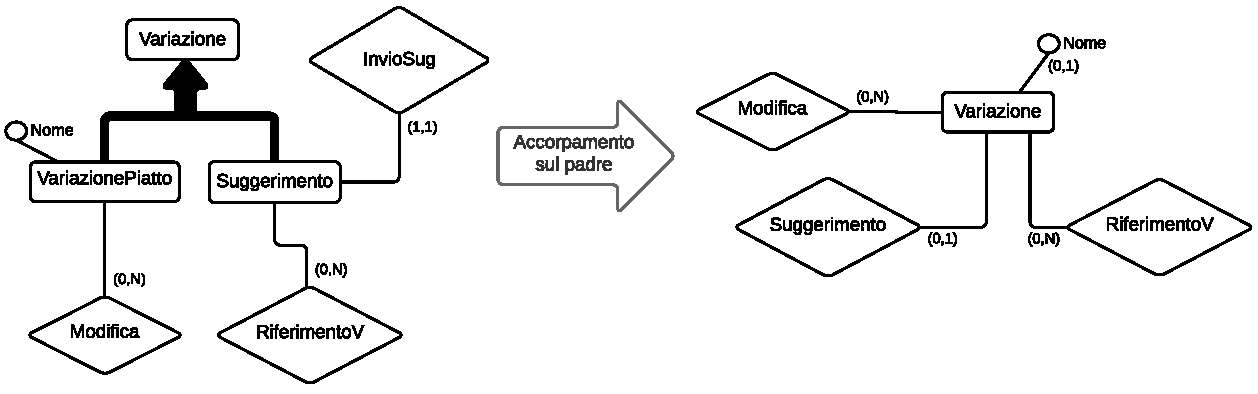
\includegraphics[width=\textwidth]{gen-variazione}}

\vspace{15pt}

Nel caso della generalizzazione che coinvolge le entità {\tt ModificaFase}, {\tt AggiuntaFase},
{\tt EliminazioneFase} e {\tt SostituzioneFase}, l'accorpamento sul padre porta all'eliminazione
di due associazioni (una {\tt Nuova} e una {\tt Vecchia}). Non è necessario introdurre qui un
attributo {\tt Tipo} per riconoscere il tipo di modifica di fase in quanto può essere facilmente
dedotto dalla presenza o meno delle associazioni {\tt Nuova} e {\tt Vecchia}: {\tt Nuova} = {\tt AggiuntaFase};
{\tt Vecchia} = {\tt EliminazioneFase}; {\tt Nuova} + {\tt Vecchia} = {\tt SostituzioneFase}.

\vspace{5pt}\centerline{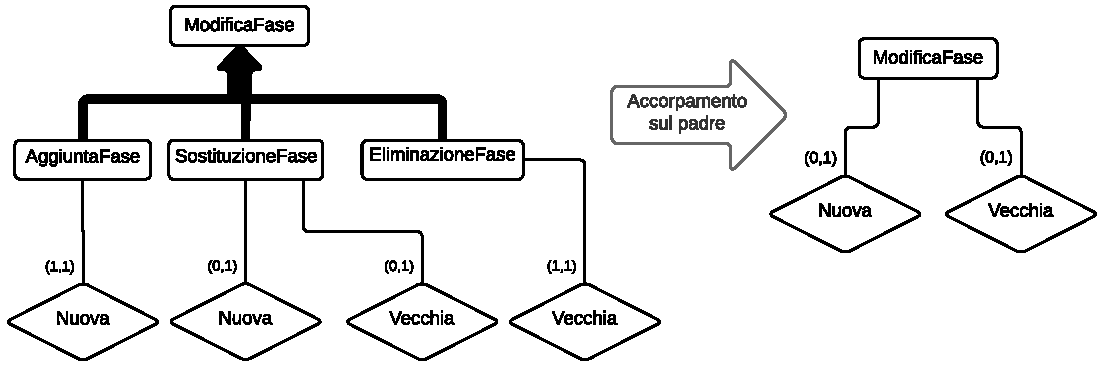
\includegraphics[width=\textwidth]{gen-modificafase}}

\vspace{15pt}

Nel caso della generalizzazione che coinvolge le entità {\tt Comanda}, {\tt ComandaTavolo}
e {\tt ComandaTakeAway}, l'accorpamento sul padre non porta all'aggiunta di attributi opzionali.
Ma le associazioni {\tt Mittente} e {\tt Ordinazione} diventano opzionali ({\tt Richiesta} è
già opzionale). Non è necessario inserire qui un attributo {\tt Tipo} per riconoscere
il tipo di comanda in quanto può essere facilmente dedotto dalla presenza o meno
dell'associazione {\tt Ordinazione}.

\vspace{5pt}\centerline{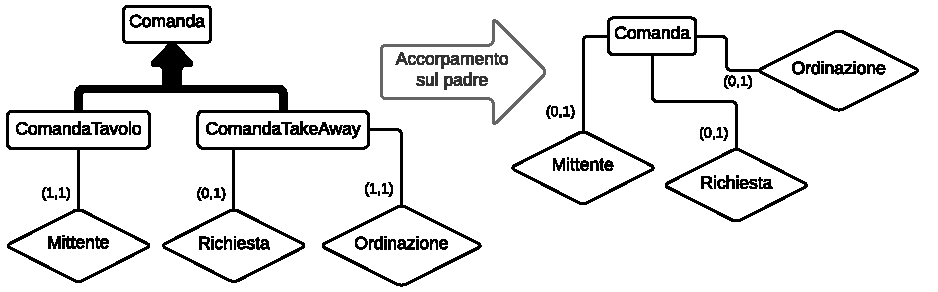
\includegraphics[width=\textwidth]{gen-comanda}}

\vspace{15pt}

Nel caso della generalizzazione che coinvolge le entità {\tt Gradimento}, {\tt GradimentoProposta}
e {\tt GradimentoSuggerimento}, l'accorpamento sul padre non porta all'aggiunta di attributi opzionali.
Ma le associazioni {\tt RiferimentoP} e {\tt RiferimentoS} diventano opzionali.
Non è necessario inserire qui un attributo {\tt Tipo} per riconoscere il tipo di
comanda in quanto può essere facilmente dedotto dall'associazione presente (se
{\tt RiferimentoP} o {\tt RiferimentoS}).

\vspace{5pt}\centerline{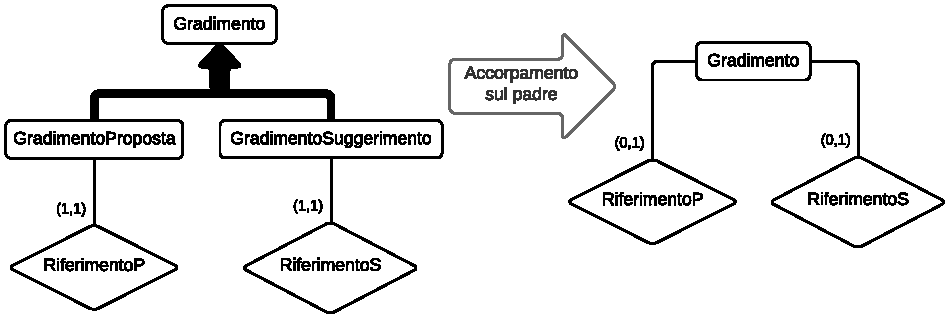
\includegraphics[width=\textwidth]{gen-gradimento}}

\vspace{15pt}

Nel caso delle due generalizzazioni che coinvolgono le entità {\tt Prenotazione},
{\tt PrenotazioneTelefonica}, {\tt PrenotazioneOnline} e {\tt Allestimento} si può
procedere con due accorpamenti sul padre: prima l'accorpamento di {\tt Allestimento}
su {\tt PrenotazioneOnline}; poi l'accorpamento di {\tt PrenotazioneTelefonica} e
{\tt PrenotazioneOnline} su {\tt Prenotazione}. Tutti gli attributi di {\tt PrenotazioneTelefonica}
e {\tt Allestimento} diventano opzionali, così anche le associazioni {\tt InvioPre}
e {\tt SerataTema}. Non è necessario inserire qui un attributo {\tt Tipo} per riconoscere
il tipo di prenotazione in quanto può essere facilmente dedotto dalla presenza o meno delle
associazioni {\tt InvioPre}, {\tt SerataTema} e {\tt Riserva}.

\vspace{5pt}\centerline{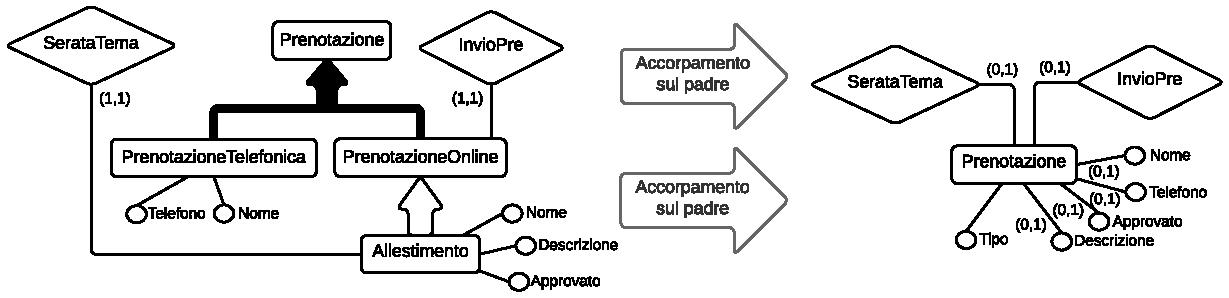
\includegraphics[width=\textwidth]{gen-prenotazione-allestimento}}
